\documentclass[border=3pt]{standalone}
\usepackage{tikz}
\usetikzlibrary{arrows.meta,calc,positioning}
\tikzset{pin/.style={-{Stealth[length=5pt]}},
  blk/.style={draw, thick, font=\sffamily\small, align=center}}
\begin{document}
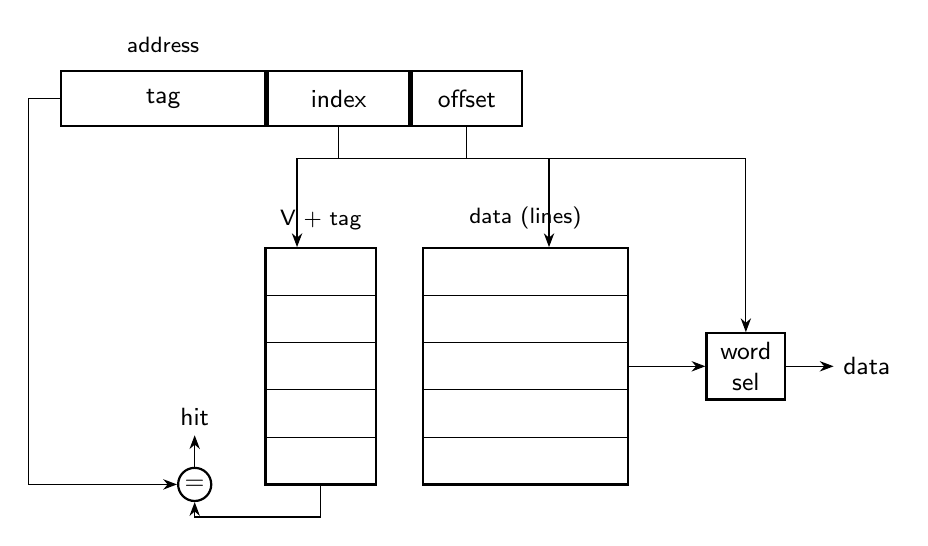
\begin{tikzpicture}[font=\sffamily\small]
  % address fields
  \node[blk, minimum width=26mm, minimum height=7mm] (tagf) at (0,0) {tag};
  \node[blk, minimum width=18mm, minimum height=7mm, anchor=west] (idxf) at (tagf.east) {index};
  \node[blk, minimum width=14mm, minimum height=7mm, anchor=west] (offf) at (idxf.east) {offset};
  \node[font=\sffamily\footnotesize, above=1mm of tagf.north] {address};
  % arrays
  \node[blk, minimum width=14mm, minimum height=30mm] (tags) at (2.0,-3.4) {};
  \node[blk, minimum width=26mm, minimum height=30mm] (data) at (4.6,-3.4) {};
  \node[font=\sffamily\footnotesize, above=1mm of tags.north] {V + tag};
  \node[font=\sffamily\footnotesize, above=1mm of data.north] {data (lines)};
  \foreach \y in {-9,-3,3,9}{
    \draw ($(tags.west)+(0,\y mm)$) -- ($(tags.east)+(0,\y mm)$);
    \draw ($(data.west)+(0,\y mm)$) -- ($(data.east)+(0,\y mm)$);}
  % index selects a row
  \draw[pin] (idxf.south) -- ++(0,-4mm) -| ($(tags.north)+(-3mm,0)$);
  \draw[pin] (idxf.south) -- ++(0,-4mm) -| ($(data.north)+(3mm,0)$);
  % comparator
  \node[draw, thick, circle, inner sep=1.5pt] (cmp) at (0.4,-4.9) {$=$};
  \draw[pin] (tagf.west) -- ++(-4mm,0) |- (cmp.west);
  \draw[pin] ($(tags.south)+(0,0)$) |- ++(-8mm,-4mm) -| (cmp.south);
  \draw[pin] (cmp.north) -- ++(0,4mm) node[above, font=\sffamily\small]{hit};
  % offset selects word
  \node[blk, minimum width=10mm, minimum height=8mm] (mux) at (7.4,-3.4) {word\\sel};
  \draw[pin] (data.east) -- (mux.west);
  \draw[pin] (offf.south) -- ++(0,-4mm) -| (mux.north);
  \draw[pin] (mux.east) -- ++(6mm,0) node[right]{data};
\end{tikzpicture}
\end{document}
